\documentclass{article}
\usepackage{amsmath}
\usepackage[pdftex]{graphicx}
\usepackage{subfigure}
\usepackage{indentfirst}

\title{Information Theoretic Modeling -- Exercise 6}
%\author{Haibo Jin}
\date{}


\bibliographystyle{plain}

\begin{document}

\maketitle

{\centering \large \textbf{Haibo Jin}}

{\centering \large \textbf{Student number: 014343698}}

\section{Problem 1}

It has been implemented in \emph{$multi\_nml.py$}. And Figure 1 shows the running result of the program.

\vspace{5mm}
\begin{minipage}{0.9\textwidth}
  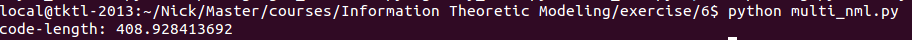
\includegraphics[width=1.1\textwidth,keepaspectratio]{1.png}
  \centerline{Figure 1: Multinomial NML.}
\end{minipage}
\vspace{5mm}




\section{Problem 2}

\subsection*{(a)}

This problem has been implemented in \emph{$bayes\_network.py$}. Figure 2 shows the running result of the program.

\vspace{5mm}
\begin{minipage}{0.9\textwidth}
  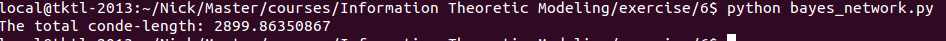
\includegraphics[width=1.1\textwidth,keepaspectratio]{2.png}
  \centerline{Figure 2: The total fNML code-length of the given bayesian network.}
\end{minipage}
\vspace{5mm}

\subsection*{(b)}

\section{Problem 3}

I first see the distributions of the word and bigrams, then simply replace the frequent ones. \emph{$data$} has the original file that to be compressed and \emph{$data.py$} has the program that can generate the file. Please see Figure 3 for the total word count before and after the compression, though it is not so efficient. 

\vspace{5mm}
\begin{minipage}{0.9\textwidth}
  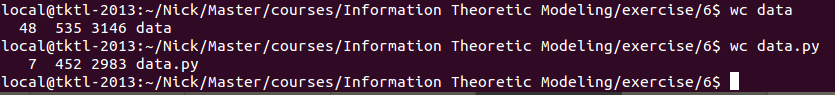
\includegraphics[width=\textwidth,keepaspectratio]{3.png}
  \centerline{Figure 3: Total word count before and after the compression.}
\end{minipage}
\vspace{5mm}

\section{Problem 4}

Please see the implementation in \emph{$google\_distance.py$}.

\subsection*{(a)}

Figure 4 shows the pairwise distance of words in the given set.

\vspace{5mm}
\begin{minipage}{0.9\textwidth}
  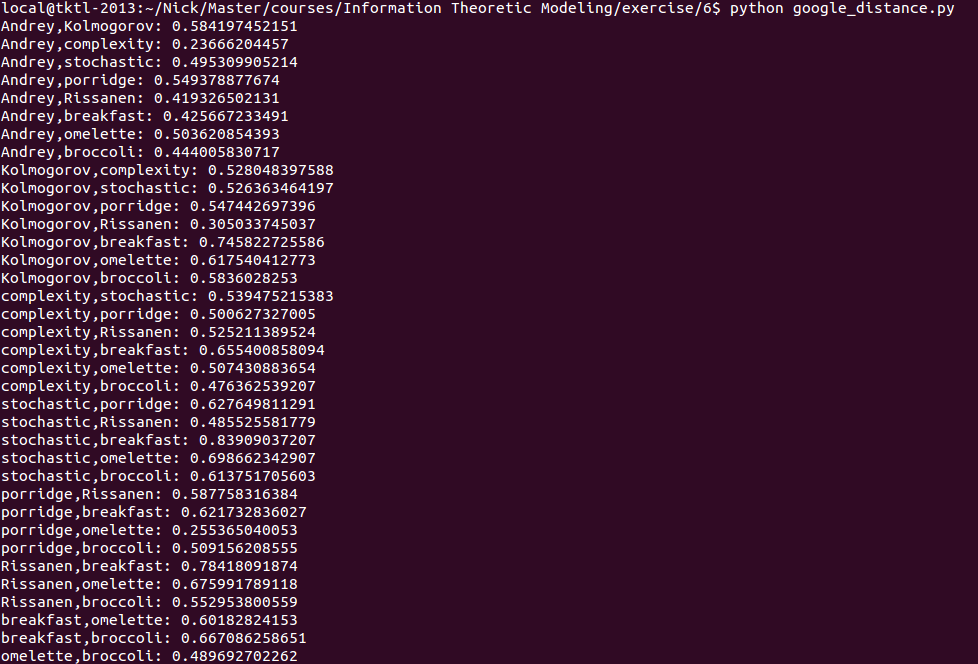
\includegraphics[width=\textwidth,keepaspectratio]{4.png}
  \centerline{Figure 4: Normalized google distance for every pair of words.}
\end{minipage}
\vspace{5mm}

\subsection*{(b)}

Figure 5 shows the heatmap of the $9 \times 9$ distance matrix. The part with cold colors indicates the distance between the two words is small while warm colors means the two words are not so close. As we can see, the distance between \emph{Andrey} and \emph{complexity} is small. The same for \emph{Kolmogorov} and \emph{Rissanen}, \emph{porridge} and \emph{omelette}. So, the NGD does indicate the semantic relatedness. However, it does not indicate all the pairs that are correlated, such as \emph{Andrey} and \emph{Kolmogorov}.

\vspace{5mm}
\begin{minipage}{0.9\textwidth}
  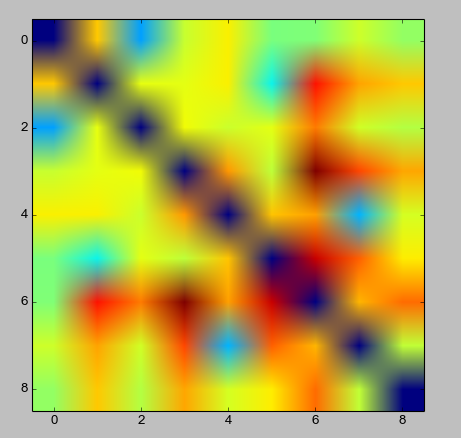
\includegraphics[width=\textwidth,keepaspectratio]{5.png}
  \centerline{Figure 5: Heatmap of the $9 \times 9$ distance matrix.}
\end{minipage}
\vspace{5mm}

\end{document}